%\documentclass[main.tex]{subfiles}
%\begin{document}

\newpage
\section{Measurements and Testing}
This chapter will summarise a number of measurements performed at CHARM, with the aim of later benchmarking the FLUKA calculated data, so that in the future we can rely confidently on the calculations, and minimise the number of measurements needed. There are a number of key areas of interest for the measurements which can be divided into the following; non-shielded test-area positions, shielded test-area positions, and the in-beam Montrac position. \\

A series of measurements were performed during 2014 and 2015 \cite{charmcalibration} using the Radmon \cite{Wijnands_radmon} detector system for dose and high-energy hadron equivalent fluence at a number of different test positions and facility configurations. A comparison has been made for the integral dose and fluence values calculated using FLUKA for respective positions, and the results for which are shown in tables \ref{tab:datatable-cpOOOO-dose}, \ref{tab:datatable-cpOOOO-heheq}, \ref{tab:datatable-cpCIIC-dose} and \ref{tab:datatable-cpCIIC-heheq}, where M/F stands for measurement divided by the value calculated with FLUKA. All the Radmon dose and HEHeq data was normalised per proton on target using the SEC1 with the calibration factor of 1.84E7 protons per count. The errors on the Radmon measurements can be assumed around 20\%. All values are an average of 3 measurements taken over 3 different test periods. \\

There is a systematic overestimate of the dose for both shielding configurations. This is likely due to the difference between scoring in air in the calculations, compared to measuring the dose in Silicon using the Radmon. Another source of error could come from any non-physical effects caused by (too high) particle energy cut-off thresholds set during the simulations.  A separate analysis is under-way to explore both these options. \\

In the case without shielding. the calculations seem able to accurately model the high-energy hadron equivalent fluence, with the ratio between measurement and calculations around 1 in table \ref{tab:datatable-cpOOOO-heheq}. One exception to this is at position 10, however this value is based on only 2 measurements. For the case with shielding, the match is less strong, showing around a 20\% overestimate of the calculations. This may be due to a difference in the way the high-energy hadron equivalent fluence is modelled in FLUKA, as the measurements were made using the V6 Radmon and the original implementation was based on the V5 Radmon system. This has a particular impact on the 'intermediate' energy neutrons, for which there is a significantly different response between the 2 detectors. \\

\begin{table}[htbp]
  \centering
    \begin{tabular}{c|r|r|r}
    \textbf{Position} & \textbf{Radmon} & \textbf{FLUKA} & \textbf{M/F} \\
    \hline
    \hline
    1     & 6.35E-15 & 1.10E-14 & 0.69 \\
    2     & 6.85E-15 & 1.21E-14 & 0.68 \\
    3     & 1.26E-14 & 2.28E-14 & 0.66 \\
    5     & 9.26E-15 & 2.11E-14 & 0.53 \\
    7     & 1.18E-14 & 2.26E-14 & 0.63 \\
    9     & 1.11E-14 & 2.07E-14 & 0.64 \\
    10    & 1.36E-14 & 2.40E-14 & 0.68 \\
    \end{tabular}%
    \caption{A table of dose measurements showing the comparison with the FLUKA calculations at various test positions for the copper target (no shielding) configuration.}
  \label{tab:datatable-cpOOOO-dose}%
\end{table}%

\begin{table}[htbp]
  \centering
    \begin{tabular}{c|r|r|r}
    \textbf{Position} & \textbf{Radmon} & \textbf{FLUKA} & \textbf{M/F} \\
    \hline
    \hline
    1     & 2.70E-05 & 3.35E-05 & 0.97 \\
    2     & 2.30E-05 & 3.49E-05 & 0.79 \\
    3     & 4.02E-05 & 5.02E-05 & 0.96 \\
    5     & 3.62E-05 & 4.34E-05 & 1.00 \\
    7     & 3.92E-05 & 4.56E-05 & 1.03 \\
    9     & 3.70E-05 & 4.17E-05 & 1.06 \\
    10    & 5.69E-05 & 4.86E-05 & 1.41 \\
    \end{tabular}%
    \caption{A table of HEHeq measurements showing the comparison with the FLUKA calculations at various test positions for the copper target (no shielding) configuration.}
  \label{tab:datatable-cpOOOO-heheq}%
\end{table}%

\begin{table}[htbp]
  \centering
    \begin{tabular}{c|r|r|r}
    \textbf{Position} & \textbf{Radmon} & \textbf{FLUKA} & \textbf{M/F} \\
    \hline
    \hline
    1     & 4.67E-16 & 6.78E-16 & 0.83 \\
    2     & 4.82E-16 & 7.57E-16 & 0.76 \\
    3     & 7.60E-16 & 1.30E-15 & 0.70 \\
    5     & 1.00E-15 & 1.74E-15 & 0.69 \\
    7     & 1.18E-15 & 2.03E-15 & 0.70 \\
    9     & 1.18E-15 & 2.74E-15 & 0.52 \\
    \end{tabular}%
    \caption{A table of dose measurements showing the comparison with the FLUKA calculations at various test positions for the copper target (full shielding) configuration.}
  \label{tab:datatable-cpCIIC-dose}%
\end{table}%

\begin{table}[htbp]
  \centering
    \begin{tabular}{c|r|r|r}
    \textbf{Position} & \textbf{Radmon} & \textbf{FLUKA} & \textbf{M/F} \\
    \hline
    \hline
    1     & 1.34E-06 & 1.86E-06 & 0.87 \\
    2     & 1.51E-06 & 2.39E-06 & 0.76 \\
    3     & 2.74E-06 & 4.54E-06 & 0.72 \\
    5     & 2.94E-06 & 5.13E-06 & 0.69 \\
    7     & 3.45E-06 & 5.55E-06 & 0.75 \\
    9     & 4.36E-06 & 6.08E-06 & 0.86 \\
    \end{tabular}%
    \caption{A table of HEHeq measurements showing the comparison with the FLUKA calculations at various test positions for the copper target (full shielding) configuration.}
  \label{tab:datatable-cpCIIC-heheq}%
\end{table}%





%\section{Non-shielded Positions}
%%Radmon data?
%%radfets
%
%\section{Shielded Positions}
%%Radmon data?
%%radfets
%
%\clearpage
%\section{Montrac Test Position}
%
%Testing at the Montrac location is typically performed without the target, which means the radiation field is dominated by the primary beam. Therefore it is only suitable for tests requiring a mono-energetic proton beam of 24 GeV. However as the dose rate and particle fluence is high, it is a good place for dose testing, radiation damage to materials, and for detector calibration purposes. \\
%
%The tests parameters are limited by the beam conditions, namely in the intensity and frequency of the spills, and the dimensions in the x and y plane. There are two main modes for the kind of beam sent to CHARM: target beam and blown-up beam conditions, shown in table X. These conditions can vary during operation, depending on the requirements for the various PS beam users. \\

% blown-up beam conditions
% % results from the alu-foils report (reference it)
% normal beam conditions
% % show example of MWPC/BPM


%Dose, HEH, 1MeV-eq n fluence in Si, beam size, gradients, peak values:
%\begin{itemize}
%	\item In-beam tests (normal beam)
%	\item In-beam tests (blown-up beam)
%	\item Tests with target
%\end{itemize}
%
%\begin{figure}[!ht]
%	\centering
%	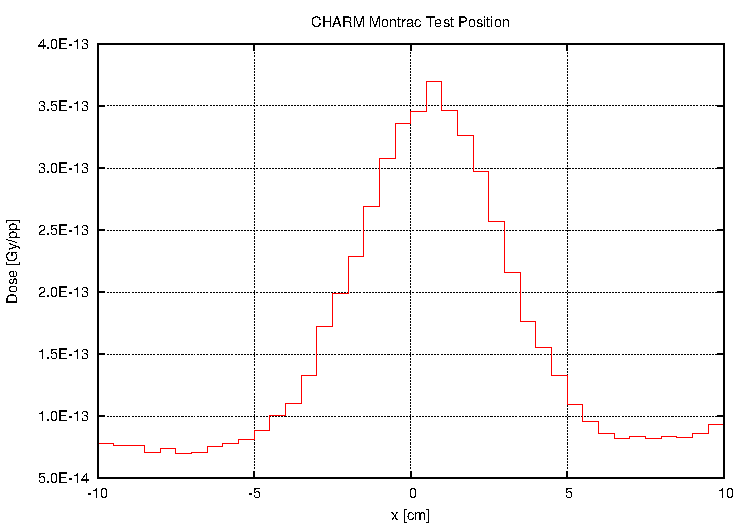
\includegraphics[width=0.45\textwidth]{./images/montrac_dose_1d_x}\quad
%	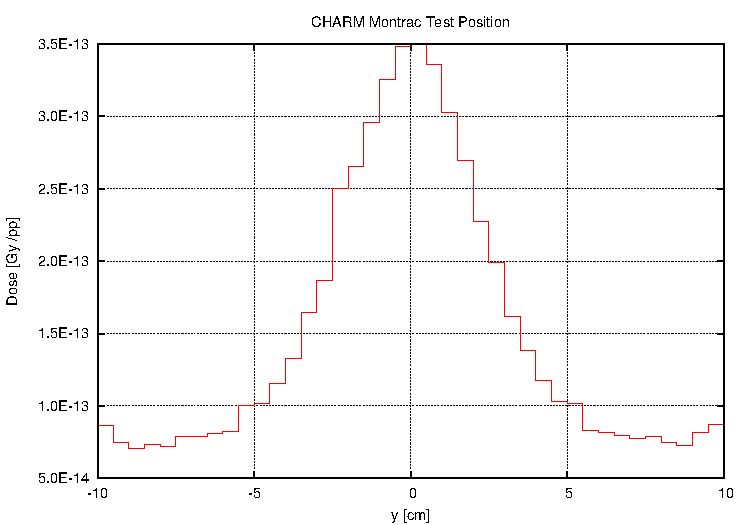
\includegraphics[width=0.45\textwidth]{./images/montrac_dose_1d_y}
%	\caption{A plot of the dose profiles per proton at the Montrac test location (in beam).}
%	\label{fig:montrac_cp_OOOO_dose}
%\end{figure}
%
%\begin{figure}[!ht]
%	\centering
%	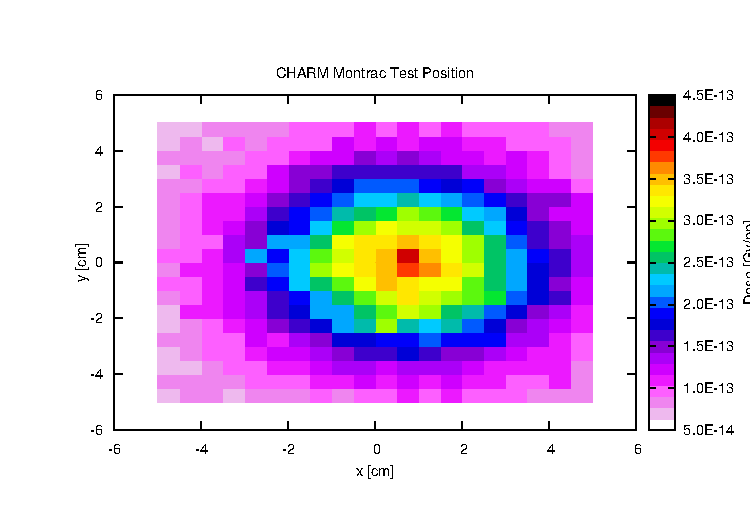
\includegraphics[width=0.7\textwidth]{./images/montrac_dose_2D}\
%	\caption{A plot of the dose per proton in 2D at the Montrac test location (in beam).}
%	\label{fig:montrac_cp_OOOO_dose_2D}
%\end{figure}

\clearpage
%\section{BLM}
%Maris' work

%plots of the normal and blown up beam from the MWPC
%alu-foils data
%esa-monitor